
\documentclass[12pt, onecolumn]{IEEEtran}
%\documentclass{article}
\usepackage[utf8]{inputenc}
\usepackage[T1]{fontenc}
\usepackage{lmodern}
\usepackage{graphicx}
\usepackage{color}
\usepackage{hyperref}
\usepackage{amsmath}
\usepackage{amsfonts}
\usepackage{epstopdf}
\usepackage[table]{xcolor}
\usepackage{matlab}
\usepackage{amssymb}
\usepackage{latexsym}
\usepackage{epsfig}
%\usepackage{comp}
\usepackage{algorithm}
\usepackage{algorithmic}

\begin{document}
	\author{Athar Ali (22915030)}
	\title{\bf{ \large EEN - 521 Digital Signal and Image Processing\\ Lab Report 2}}
	\maketitle 
	\markboth{\small \it{D\lowercase{epartment of} E\lowercase{lectrical} E\lowercase {ngineering}}  \hfill A\lowercase{utumn} S\lowercase{emester 
			2022} } {}
	
	%\matlabheading{EEN - 521 Digital Signal and Image Processing}
	
	
	\vspace{1em}
	\begin{par}
		\begin{flushleft}
			\textbf{1) Construct a signal $\mathbf{y = sin((n\pi/10)n) + 10 sin(n\pi/50) + 20 sin(n\pi/100), \ for \ \ n = \ {0, 1, 2, ,...200}}$. Add 50 zeros at both of the ends of signal sample. Construct an averaging window of 50 length and unity strength throughout. Further, impose this averaging window to the mentioned signal, and plot the input and output of the signal.} 
		\end{flushleft}
	\end{par}
	
	\begin{matlabcode}
		clc; % clearing screen
		clear; % clearing previos variables 
		close all % closing previos windows   
		
		
		n=0:200; % Indices
		yn=sin(n.*n*pi/10)+10*sin(n*pi/50)+20*sin(n*pi/100); % Input Sequence
		y1n=[zeros(1,50) yn zeros(1,50)]; % Padding Zeros
		filterd_Seq=movmean(y1n,50); % Filtering    
		
		figure
		stem(y1n,'filled'); % plotting Input Sequence
		xlabel('n'); 
		ylabel('y(n)');
		title('Plot of Sequence,in(n*pi/10)+10*sin(n*pi/50)+20*sin(n*pi/100)');
	\end{matlabcode}
\begin{center}
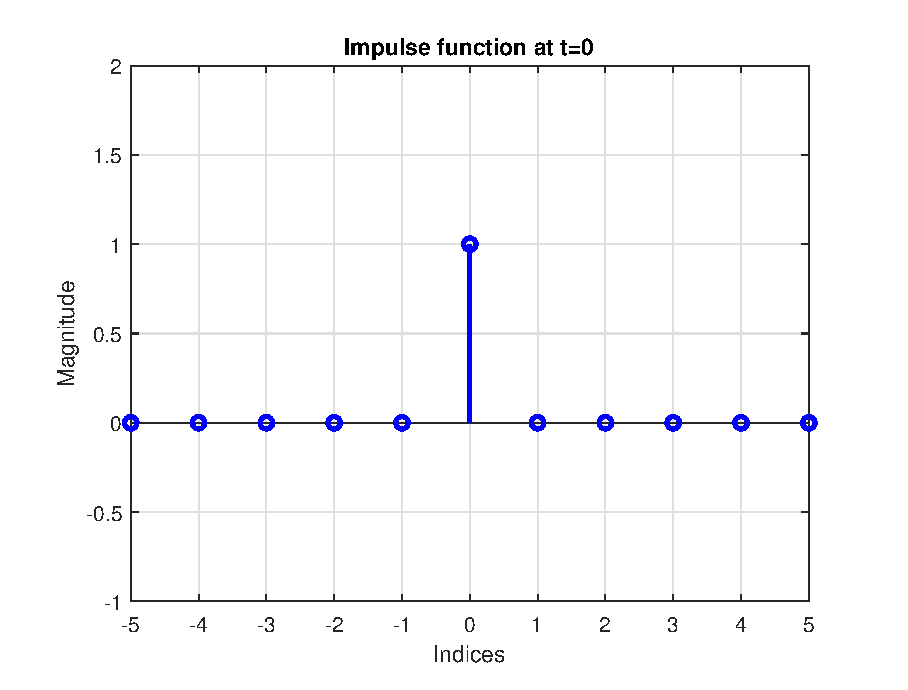
\includegraphics[width=\maxwidth{56.196688409433015em}]{figure_0.eps}
\end{center}
\begin{matlabcode}

figure
stem(filterd_Seq,'filled'); % Plotting Filtered Sequence 
xlabel('n'); 
ylabel('y(n)');
title('Plot of Sequence, after applying average filter');
\end{matlabcode}
\begin{center}
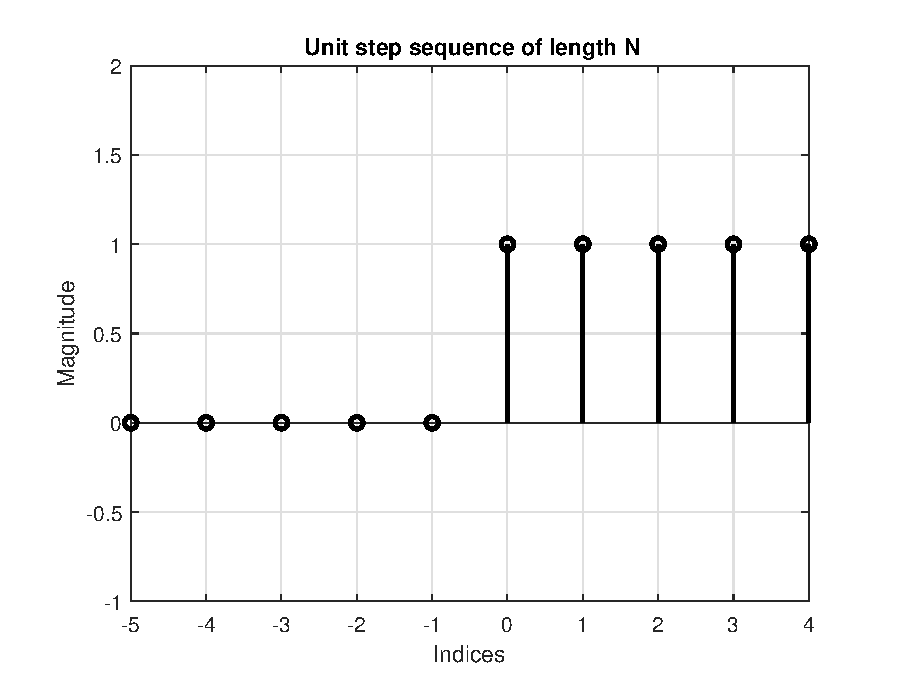
\includegraphics[width=\maxwidth{56.196688409433015em}]{figure_1.eps}
\end{center}

\begin{par}
	\begin{flushleft}
		\textbf{2) Generate a signal s[n] = 2[n(0.9)n ], for n = \{0, 1, 2, ...50\}. Corrupt s[n] with an impulse noise d[n]. Apply a median filter of length-3 to the corrupted signal s[n] + d[n] and plot the median filtered signal. Increase the median filter length to 5 and 7 and comment on your results.}
	\end{flushleft}
\end{par}

\begin{matlabcode}
	n = 0:50; % Indices 
	sn = 2*(n.*(0.9).^n); % Sequence 
	dn = 50*[n-20==0]+70*[n-40==0]; % Creating Impulsive Noise
	xn = sn + dn; % Adding Sequence
	mfs3=movmedian(xn,3);
	mfs5=movmedian(xn,5);
	mfs7=movmedian(xn,7);
	
	figure
	plot(sn,'linewidth',2); grid; % Plotting Sequence 
	xlabel('n'); 
	ylabel('s(n)');
	title('Plot of Sequence, s[n] = 2[n(0.9)^n]');
\end{matlabcode}
\begin{center}
	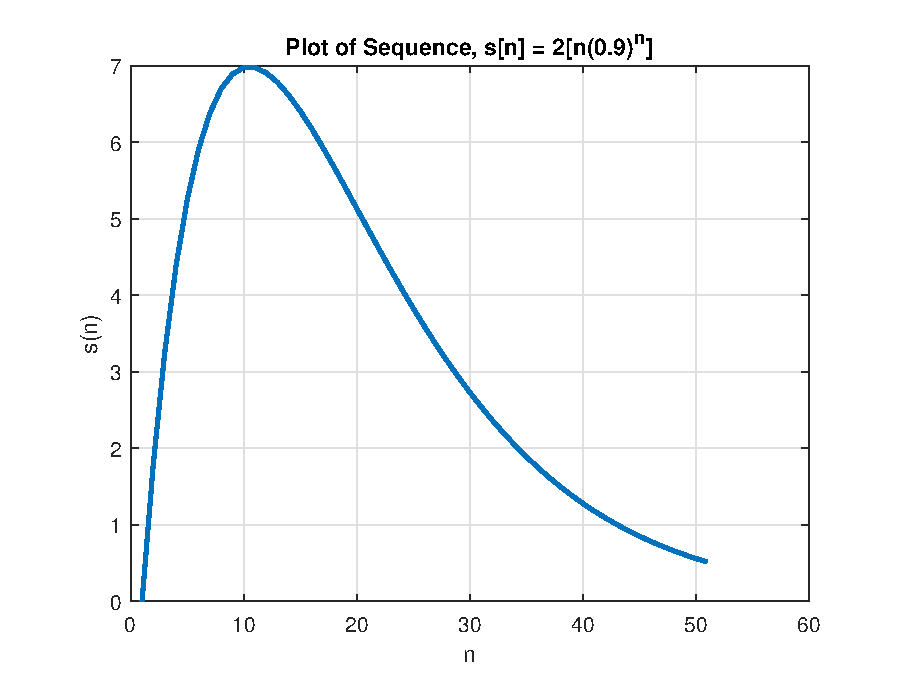
\includegraphics[width=\maxwidth{56.196688409433015em}]{figure_2.eps}
\end{center}
\begin{matlabcode}
	
	figure
	plot(dn,'linewidth',2); grid; % Plotting Noise 
	xlabel('n'); 
	ylabel('d(n)');
	title('Impulsive Noise');
\end{matlabcode}
\begin{center}
	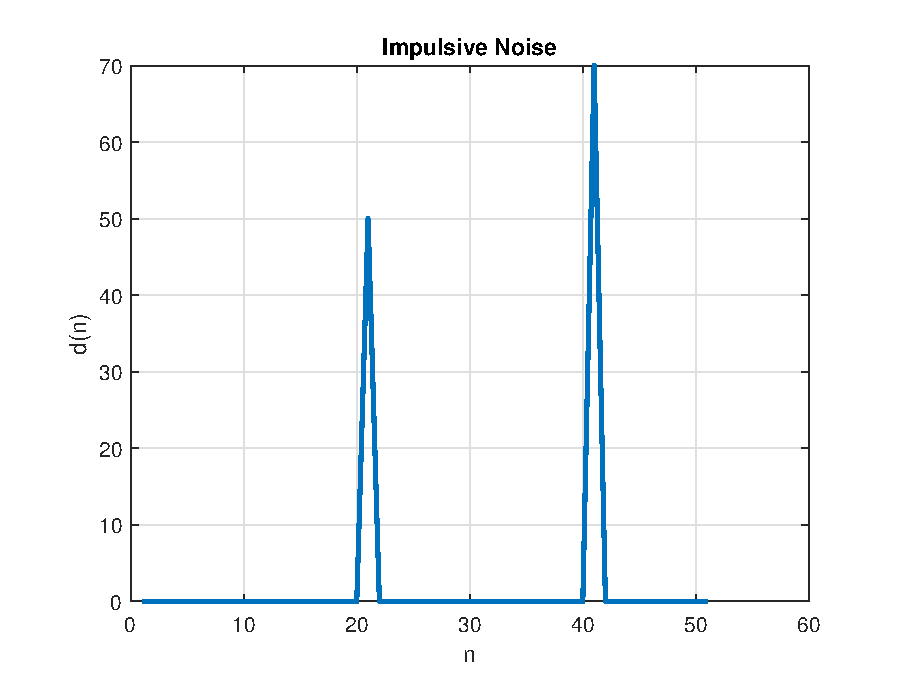
\includegraphics[width=\maxwidth{56.196688409433015em}]{figure_3.eps}
\end{center}
\begin{matlabcode}
	
	figure; 
	subplot(221)
	plot(xn,'linewidth',2); grid; % Plotting Noisey Sequence
	xlabel('n'); 
	ylabel('x(n)');
	title('Noisy Signal');
	axis([-5 60 -1 8]);
	subplot(222);
	plot(mfs3,'linewidth',2); grid; % Plotting Filterd Sequence with kernal 3x3.
	xlabel('n'); 
	ylabel('x(n)');
	title('Median Filtered Signal with kernel size 3x3');
	subplot(223);
	plot(mfs5,'linewidth',2); grid; % Plotting Filterd Sequence with kernal 5x5.
	xlabel('n'); 
	ylabel('x(n)');
	title('Median Filtered Signal with kernel size 5x5');
	subplot(224);
	plot(mfs7,'linewidth',2); grid; % Plotting Filterd Sequence with kernal 7x7.
	xlabel('n'); 
	ylabel('x(n)');
	title('Median Filtered Signal with kernel size 7x7');
\end{matlabcode}
\begin{center}
	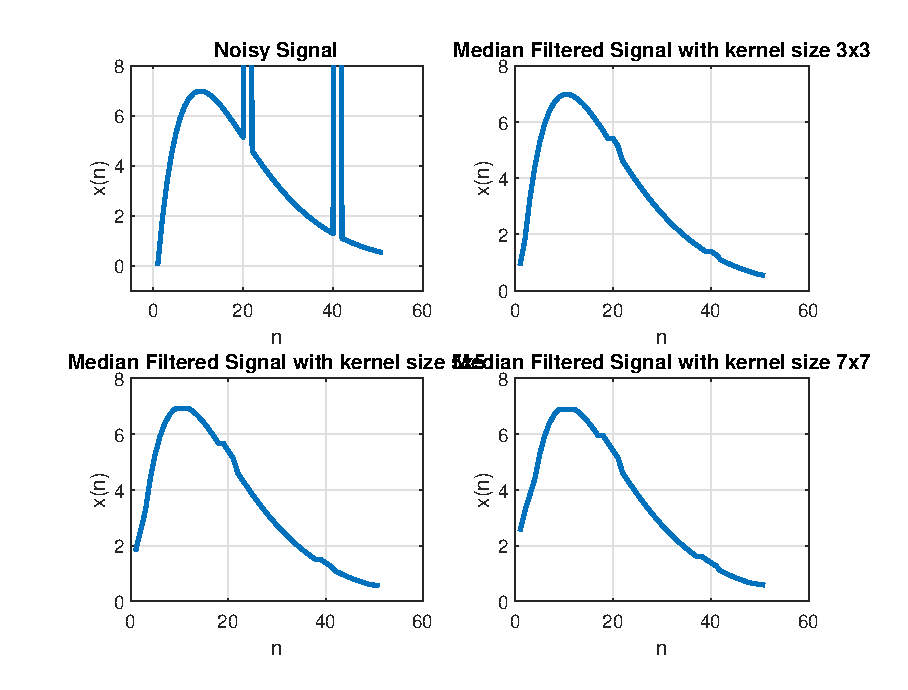
\includegraphics[width=\maxwidth{56.196688409433015em}]{figure_4.eps}
\end{center}

\begin{par}
	\begin{flushleft}
		\textbf{3) Determine the impulse and step responses of the causal LTI system given by y[n] + 0.7y[n-1]-0.45y[n-2]-0.6y[n-3] = 0.8x[n]-0.44x[n-1 + 0.36x[n-2] + 0.02x[n-3]}
	\end{flushleft}
\end{par}

\begin{matlabcode}
	% filter Designing
	n=0:50; % Indices 
	b=[0.8,-0.44,0.36,0.02]; % Filter's Numerator's Coefficients 
	a=[1,0.7,-0.45,-0.6]; % Filter's Denomonators's Coefficients 
	
	imp=[n==0]; % Impuse
	imp_resp=filter(b,a,imp); % Impuse Responce
	u = [n>=0]; % Unit Step fuction
	step_resp=filter(b,a,u); % Step responce
	
	figure; stem(imp,'linewidth',2); grid; ylim([-1 2]); % Plotting Impulse
	xlabel('n'); ylabel('del(n)'); title('Impulse at n=0'); 
\end{matlabcode}
\begin{center}
	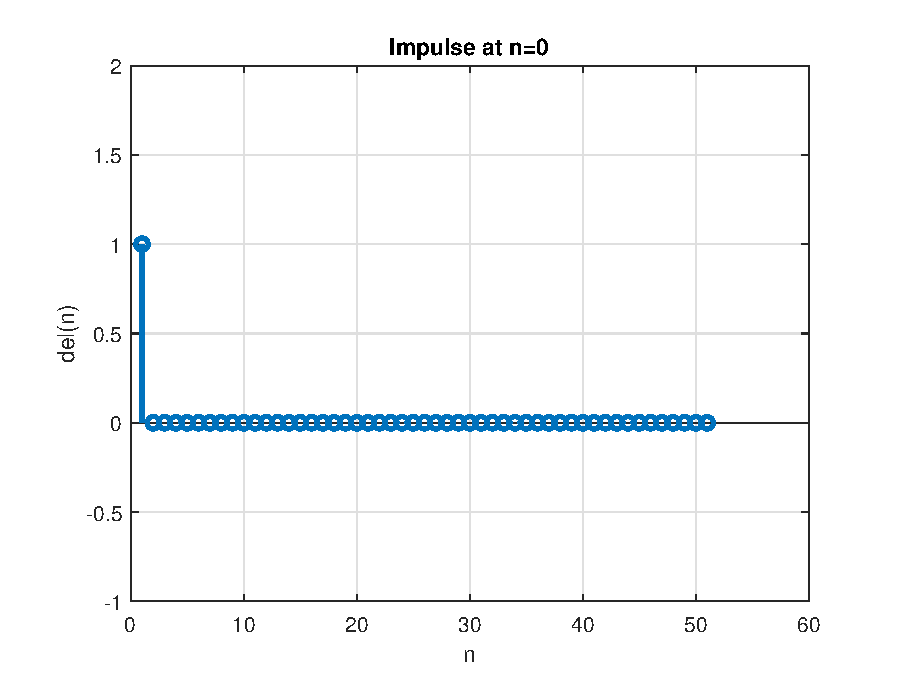
\includegraphics[width=\maxwidth{56.196688409433015em}]{figure_5.eps}
\end{center}
\begin{matlabcode}
	
	figure;stem(imp_resp,'linewidth',2); grid; % Plotting Impulse Responce
	xlabel('n'); ylabel('x(n)'); title('Impuse Responce of filter');
\end{matlabcode}
\begin{center}
	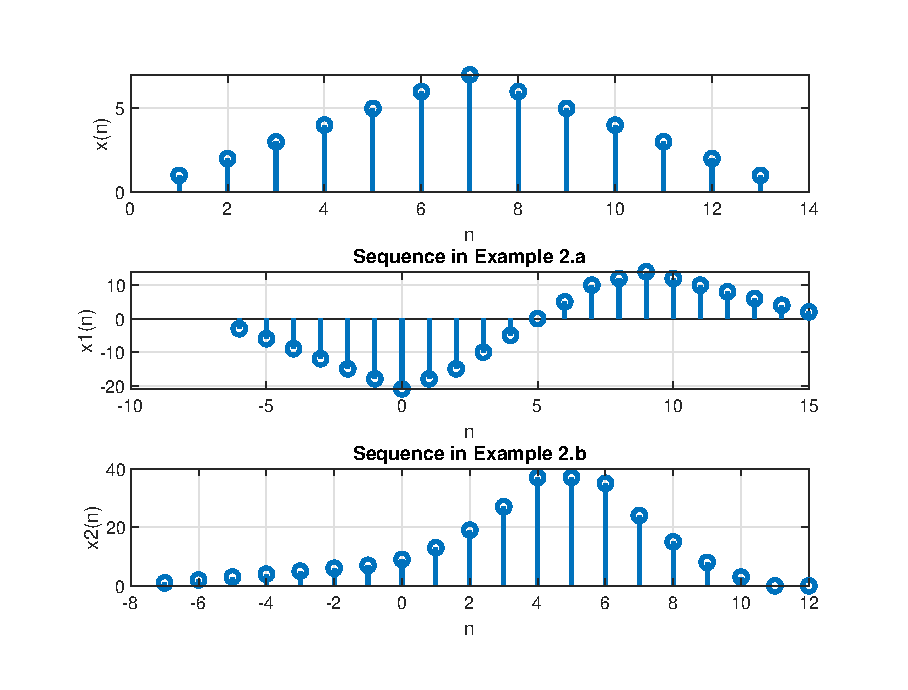
\includegraphics[width=\maxwidth{56.196688409433015em}]{figure_6.eps}
\end{center}
\begin{matlabcode}
	
	figure; stem(u,'linewidth',2); grid; % Plotiing Unit Step Function
	xlabel('n'); ylabel('del(n)'); title('Unit step fuction');
\end{matlabcode}
\begin{center}
	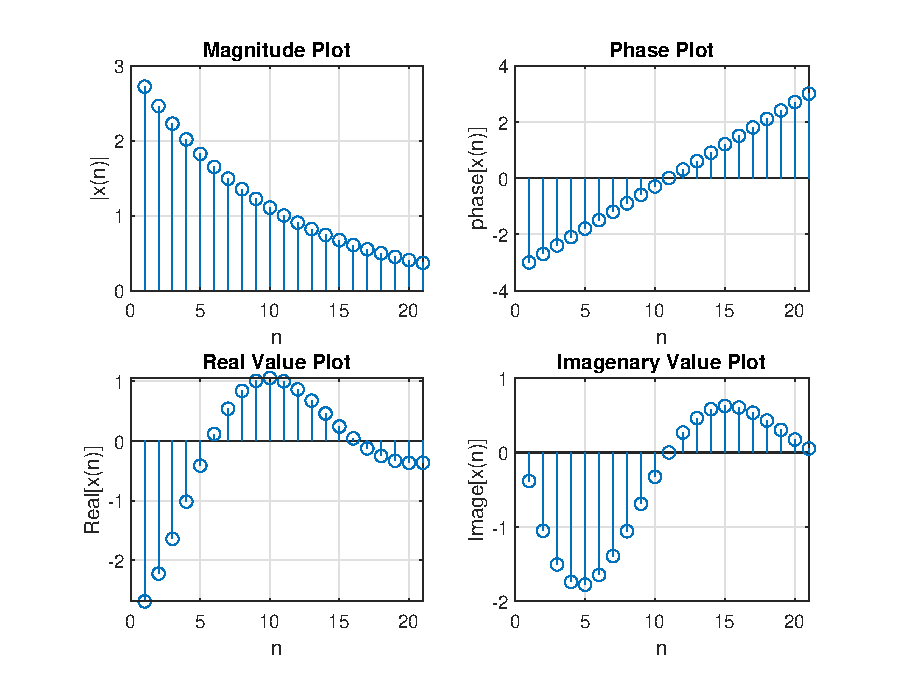
\includegraphics[width=\maxwidth{56.196688409433015em}]{figure_7.eps}
\end{center}
\begin{matlabcode}
	
	figure; stem(step_resp,'linewidth',2); grid; % Plotting Step Responce
	xlabel('n'); ylabel('x(n)'); title('Step Responce of filter');
\end{matlabcode}
\begin{center}
	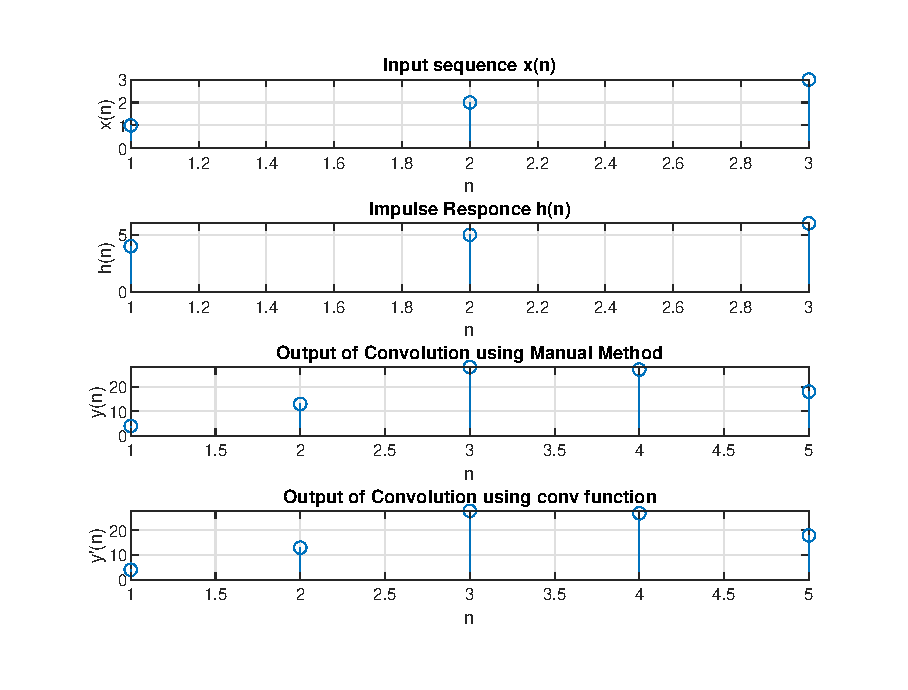
\includegraphics[width=\maxwidth{56.196688409433015em}]{figure_8.eps}
\end{center}


\begin{par}
	\begin{flushleft}
		\textbf{4) Use MATLAB function “filter” \& “filtic”, to obtain system response for a difference equation y[n] - 1.143y[n - 1] + 0.4128y[n - 2] = 0.0675x[n] + 0.1349x[n - 1] + 0.675x[n - 2] Initial conditions y[-1] = 1; y[-2] = 2.}
	\end{flushleft}
\end{par}

\begin{matlabcode}
	% Filter Designing
	b=[0.0675, 0.1349, 0.675];  % Filter's Numerator's Coefficients 
	a=[1,-1.143, 0.4128]; % Filter's Denomonators's Coefficients 
	yn=[1,2]; % Initial Values 
	ic = filtic(b,a,yn); % Inicial Conditions 
	
	imp=[n==0]; % Impuse
	imp_resp = filter(b,a,imp,ic) % Impuse Responce
\end{matlabcode}

\begin{matlabcode}
	u = [n>=0]; % Unit Step fuction
	step_resp = filter(b,a,double(u),ic); % Step responce
	
	figure;stem(imp_resp,'linewidth',2); grid; % Plotting Impulse Responce
	xlabel('n'); ylabel('x(n)');title('Impuse Responce of filter');
\end{matlabcode}
\begin{center}
	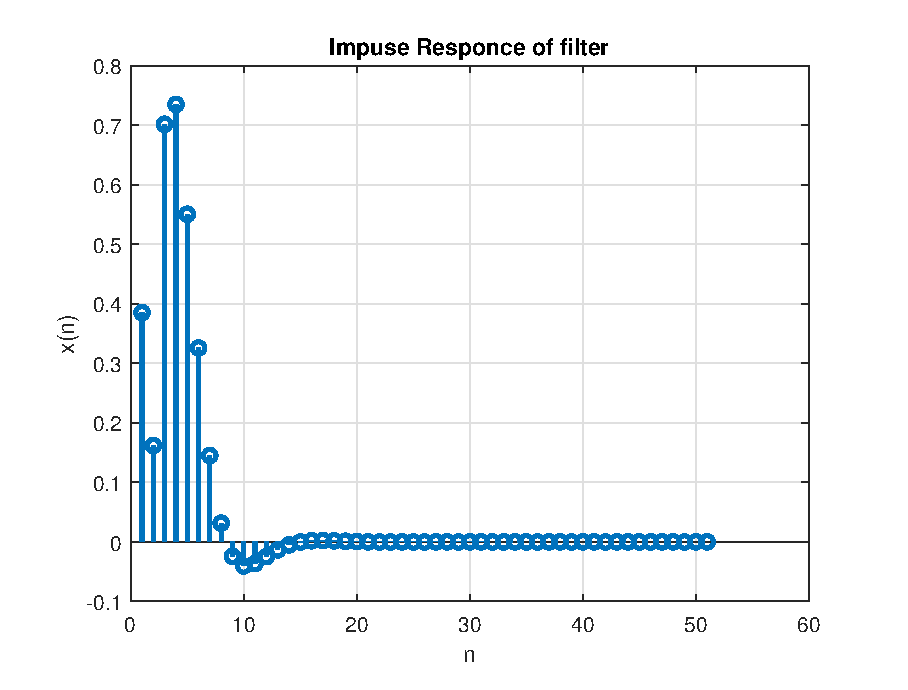
\includegraphics[width=\maxwidth{56.196688409433015em}]{figure_9.eps}
\end{center}
\begin{matlabcode}
	
	figure;stem(step_resp,'linewidth',2); grid;  % Plotting Step Responce
	xlabel('n'); ylabel('x(n)');title('Step Responce of filter');
\end{matlabcode}
\begin{center}
	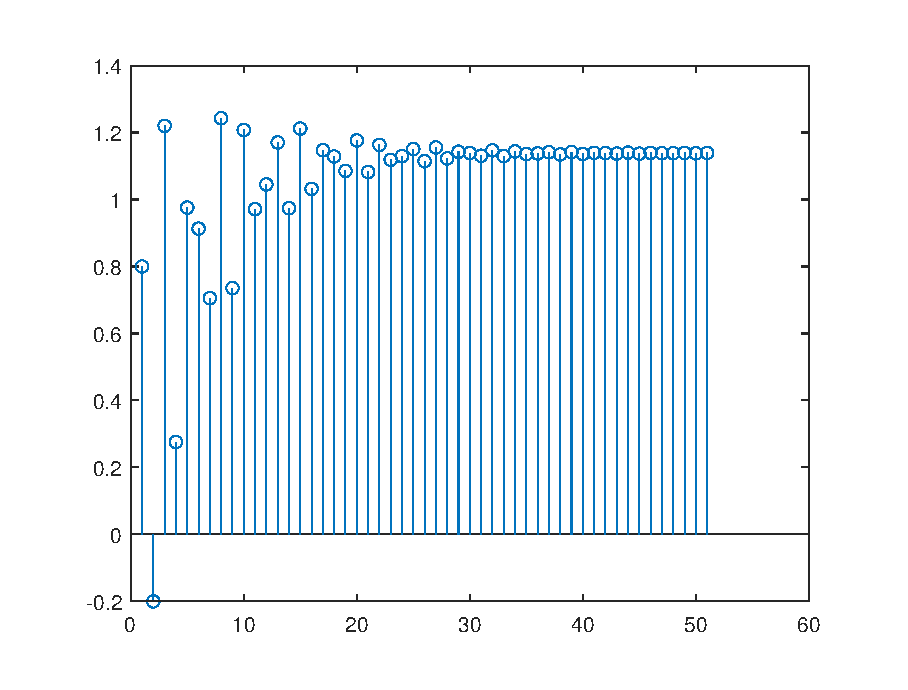
\includegraphics[width=\maxwidth{56.196688409433015em}]{figure_10.eps}
\end{center}

\begin{par}
	\begin{flushleft}
		\textbf{5) Evaluate the frequency response at the frequency $\omega  = \pi/3$ and 50 values of the steady state output in response to a complex sinusoidal input of frequency $\omega  = \pi/3$ for the moving average system with impulse response $h[n] = ( 1/4 \ \ if \ 0 \leq  n \leq  3, \ \ 0 \ otherwise$}
	\end{flushleft}
\end{par}

\begin{matlabcode}
	n=0:49; % Indices 
	len=length(n);
	hn=[ones(1,4)/4 zeros(1,len-4)]; % Impulse Responce
	xn=exp(j*len*pi/3); % Complex sinosoidal Input  
	len2=length(xn);
	
	Xw=conv(xn,hn); % Concolving the input sequence with impulse responce.
	Yw=fft(Xw); % Calculating fourier transform of convolved sequence.
	w=0:pi/49:pi; % frequency range
	
	figure; subplot(2,1,1);
	plot(w,abs(Yw),'linewidth',2); grid; % plotting magnitude of spectrum of convolved sequence.
	ylabel('Magnitude H(w)'); xlabel('Digital frequency \omega');
	title('Magnitude response |H(exp(j*w))|');
	subplot(2,1,2);
	plot(w,angle(Yw),'linewidth',2); grid; % plotting phase of spectrum of convolved sequence.
	ylabel('Phase(rad)'); xlabel('Digital frequency \omega');
	title('Phase response <H(exp(j*w))');
\end{matlabcode}
\begin{center}
	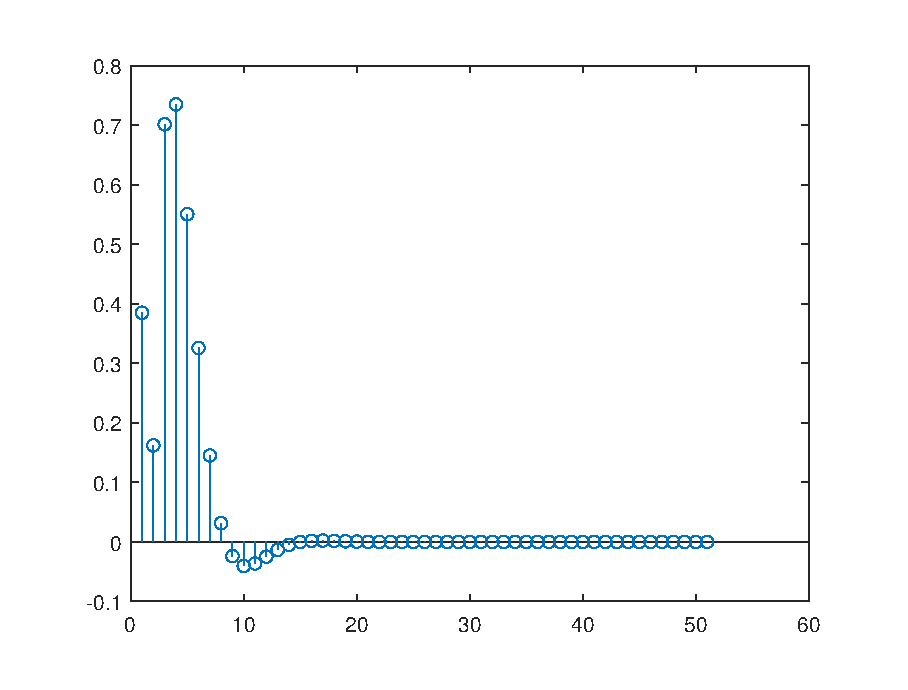
\includegraphics[width=\maxwidth{56.196688409433015em}]{figure_11.eps}
\end{center}

\begin{par}
	\begin{flushleft}
		\textbf{6) Use MATLAB to determine the DTFS coefficients of N- periodic square wave. For period N = 50 and (a) M = 12 (b) M = 5 (c) M = 20 x[n] = ( 1 if -M \textless{} n \textless{} M 0 if M \textless{} n \textless{} N - M}
	\end{flushleft}
\end{par}

\begin{matlabcode}
	N=50; % period 
	n=-N/2:N/2-1; % Range for time indices 
	k=-N/2:N/2-1; % Range of frequency indices                                          
	M=[12,5,20]; % Length of sequences for the different cases.
	
	figure
	for i=1:3
	len1=2*M(i)+1; % length of ones
	len0=N/2-M(i); % length of zeros
	xn=[zeros(1,len0) ones(1,len1) zeros(1,len0-1)]; % Sequence
	Xk=(1/N)*xn*exp(-1j*2*pi.*k.*n'/N); % DTFS of sequence.
	
	subplot(3,3,i);
	stem(n,xn); % plotting time domain sequence
	xlabel('samples (n)');
	ylabel('x(n)');
	title(['Sequence in time domain for M= ' num2str(M(i))]);
	
	subplot(3,3,i+3);
	stem(k,abs(Xk)); % plotting magnitude of spectrum
	xlabel('samples (n)');
	ylabel('|X(k)|');
	title(['Magnitude plot of DTFS coefficients for M= ' num2str(M(i))]);
	subplot(3,3,i+6)
	stem(k,angle(Xk)); % plotting phase of spectrum
	xlabel('samples (n)');
	ylabel('Phase{X(k)}');
	title(['Phase plot of DTFS coefficients for M = ' num2str(M(i))]);
	end
\end{matlabcode}
\begin{center}
	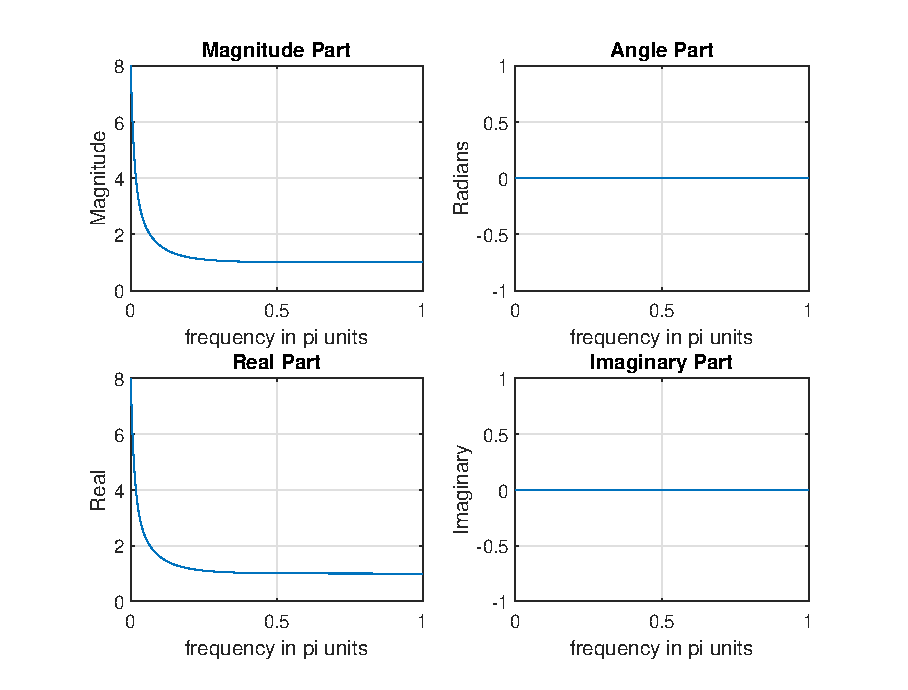
\includegraphics[width=\maxwidth{56.196688409433015em}]{figure_12.eps}
\end{center}

\begin{par}
	\begin{flushleft}
		\textbf{ \\ 7) Use MATLAB’s “fft” \& “ifft” commands to evaluate DTFS coefficients \& time-domain signal of the following  $\mathbf{(a) \ x[n] = cos( (6\pi/17)n+\pi/3) \ , \ (b) \ X[k] = cos( 8\pi k/21 )}$}
	\end{flushleft}
\end{par}

\begin{matlabcode}
	n=0:50; % indices 
	xn=cos(6*pi*n/17+pi/3); % Time domain Sequence, x(n).
	Xw=fft(xn); % Fourier Transform of sequence x(n).
	xn1=ifft(Xw); % Inverse Fourier Transform of X(w).
	
	figure; subplot(311)
	stem(n,xn); grid; % plotting the time domain sequence
	xlabel('n'); ylabel('x(n)');
	title('Time Domain Sequence, x(n) = cos(6*pi*n/17+pi/3)');
	subplot(312); k=0:50;
	stem(k,abs(Xw), 'k', 'lineWidth',2); grid; % Magnitude plot of spectrum.
	xlabel('n'); ylabel('|X(\omega)|');
	title('Magnitude plot of spectrum, X(\omega)')
	subplot(313);
	stem(n,xn1, 'r'); grid; % plotting Inverse fourier transform.
	xlabel('n'); ylabel('x1(n)');
	title('Plot of x1(n), Inverse Transform of X(\omega)');
\end{matlabcode}
\begin{center}
	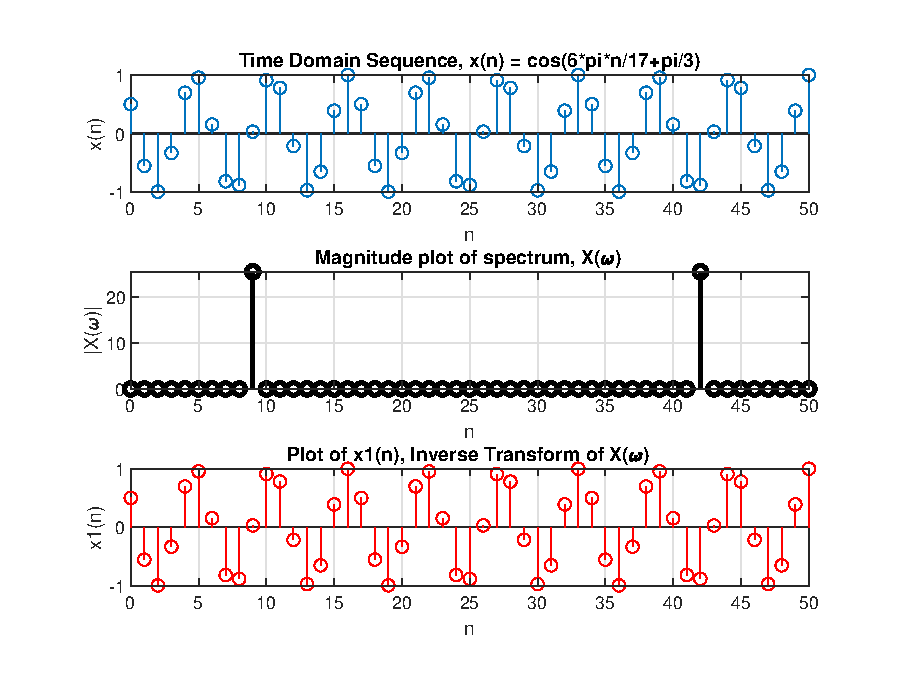
\includegraphics[width=\maxwidth{56.196688409433015em}]{figure_13.eps}
\end{center}

\begin{par}
	\begin{flushleft}
		\textbf{8) Find the DTFT of the discrete-time rectangular pulse $\mathbf{x[n] = ( 1 \ if -4 \textless{} n \textless{} 4 \ ; \ 0,}$ otherwise Using “fft”}
	\end{flushleft}
\end{par}

\begin{matlabcode}
	n=-6:6; % Indices
	xn5= [(n+3) >= 0]-[(n-3) >= 0]; % Sequence
	DTFT=fft(xn5);
	
	figure;
	stem(n,xn5,'filled','linewidth',2); grid; % plotting time domain sequence
	xlabel('n'); ylabel('x5(n)'); axis([-6 6 -1 2])
	title('Time Domain Sequence x5(n)');
\end{matlabcode}
\begin{center}
	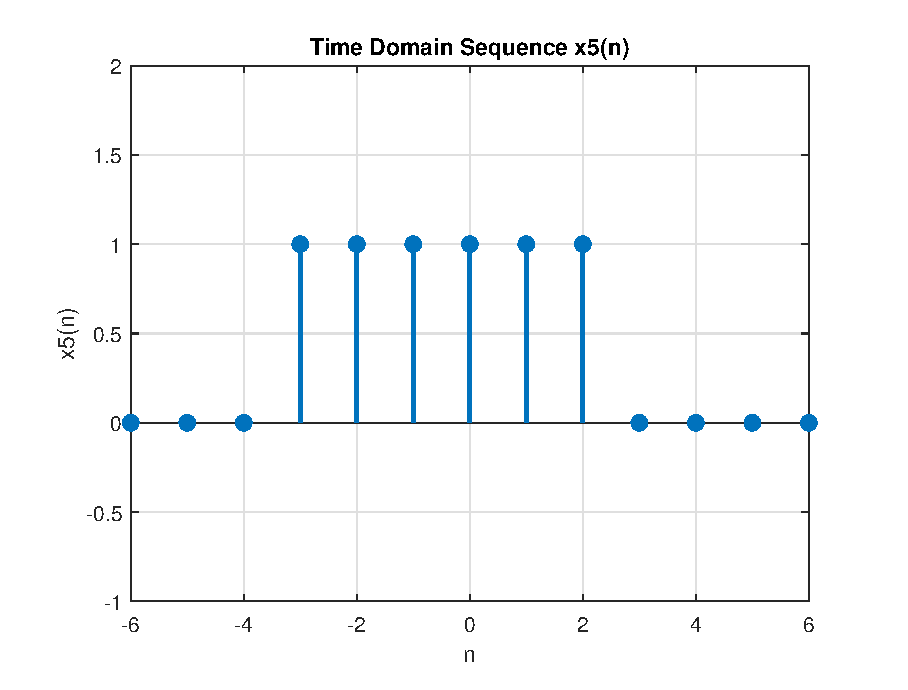
\includegraphics[width=\maxwidth{56.196688409433015em}]{figure_14.eps}
\end{center}
\begin{matlabcode}
	
	figure;
	stem(abs(DTFT),'filled','linewidth',2); grid
	xlabel('n'); 
	ylabel('X(k)');
	title('Magnitude plot of DFT of x5(n)');
\end{matlabcode}
\begin{center}
	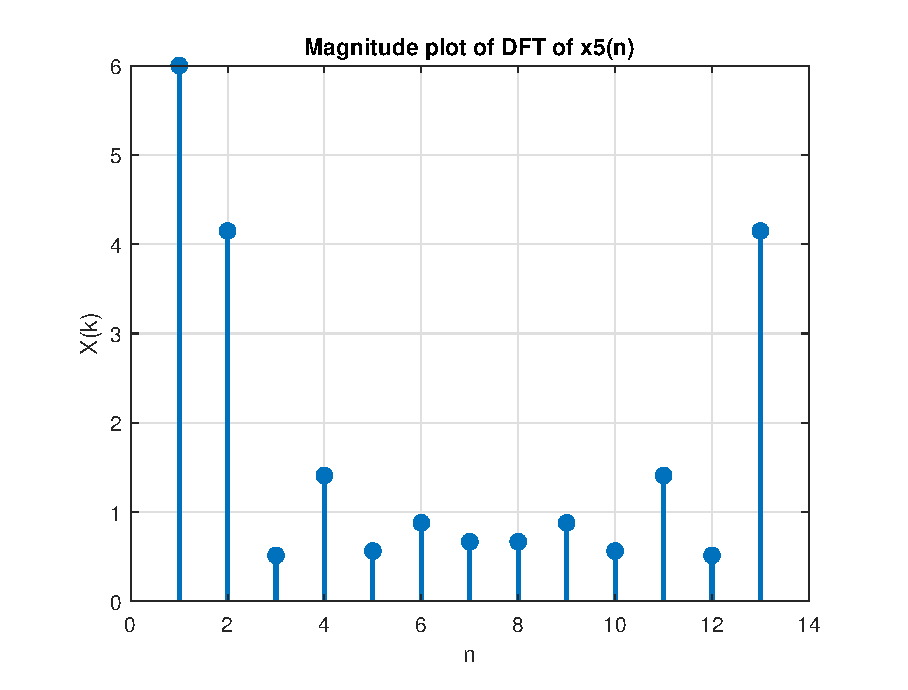
\includegraphics[width=\maxwidth{56.196688409433015em}]{figure_15.eps}
\end{center}
\begin{matlabcode}
	
	figure;
	stem(angle(DTFT),'filled','linewidth',2); grid; % plotting phase spectrum
	xlabel('n'); ylabel('X(k)');
	title('Phase plot of DFT of x5(n)');
\end{matlabcode}
\begin{center}
	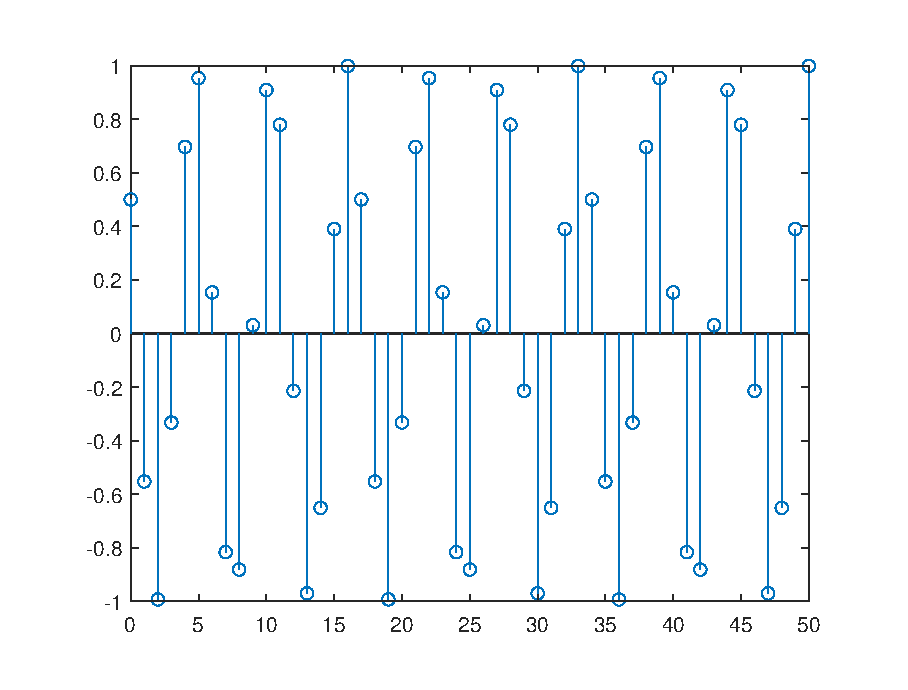
\includegraphics[width=\maxwidth{56.196688409433015em}]{figure_16.eps}
\end{center}





\end{document}
